% Generated by scripts/agents/plot_risk_coverage.py from b1_selective_prediction.json. Do not edit by hand.
% Needs \usepackage{pgfplots} and \pgfplotsset{compat=1.17} in the preamble.
\definecolor{rcseries}{HTML}{2A78D6}
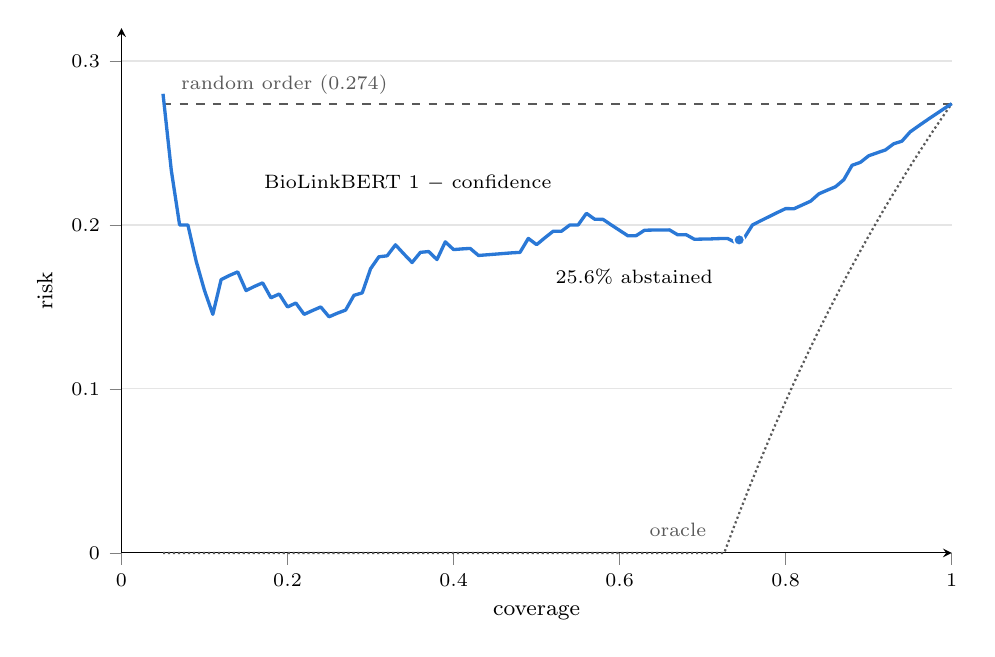
\begin{tikzpicture}
\begin{axis}[
  width=\columnwidth, height=0.68\columnwidth,
  xmin=0, xmax=1, ymin=0, ymax=0.32,
  xtick={0,0.2,0.4,0.6,0.8,1}, ytick={0,0.1,0.2,0.3},
  xlabel={coverage}, ylabel={risk},
  ymajorgrids, grid style={gray!20},
  axis lines=left, tick align=outside,
  label style={font=\footnotesize}, tick label style={font=\scriptsize},
  clip=false,
]
\addplot[gray!70!black, dashed, thick, domain=0.05:1, samples=2] {0.274};
\addplot[gray!70!black, densely dotted, thick] coordinates {(0.05,0) (0.726,0) (0.728,0.0027) (0.738,0.0163) (0.748,0.0294) (0.758,0.0422) (0.768,0.0547) (0.778,0.0668) (0.788,0.0787) (0.798,0.0902) (0.808,0.1015) (0.818,0.1125) (0.828,0.1232) (0.838,0.1337) (0.848,0.1439) (0.858,0.1538) (0.868,0.1636) (0.878,0.1731) (0.888,0.1824) (0.898,0.1915) (0.908,0.2004) (0.918,0.2092) (0.928,0.2177) (0.938,0.2260) (0.948,0.2342) (0.958,0.2422) (0.968,0.2500) (0.978,0.2577) (0.988,0.2652) (0.998,0.2725) (1.000,0.2740)};
\addplot[rcseries, very thick, line join=round] coordinates {(0.050,0.2800) (0.060,0.2333) (0.070,0.2000) (0.080,0.2000) (0.090,0.1778) (0.100,0.1600) (0.110,0.1455) (0.120,0.1667) (0.130,0.1692) (0.140,0.1714) (0.150,0.1600) (0.160,0.1625) (0.170,0.1647) (0.180,0.1556) (0.190,0.1579) (0.200,0.1500) (0.210,0.1524) (0.220,0.1455) (0.230,0.1478) (0.240,0.1500) (0.250,0.1440) (0.260,0.1462) (0.270,0.1481) (0.280,0.1571) (0.290,0.1586) (0.300,0.1733) (0.310,0.1806) (0.320,0.1812) (0.330,0.1879) (0.340,0.1824) (0.350,0.1771) (0.360,0.1833) (0.370,0.1838) (0.380,0.1789) (0.390,0.1897) (0.400,0.1850) (0.410,0.1854) (0.420,0.1857) (0.430,0.1814) (0.440,0.1818) (0.450,0.1822) (0.460,0.1826) (0.470,0.1830) (0.480,0.1833) (0.490,0.1918) (0.500,0.1880) (0.510,0.1922) (0.520,0.1962) (0.530,0.1962) (0.540,0.2000) (0.550,0.2000) (0.560,0.2071) (0.570,0.2035) (0.580,0.2034) (0.590,0.2000) (0.600,0.1967) (0.610,0.1934) (0.620,0.1935) (0.630,0.1968) (0.640,0.1969) (0.650,0.1969) (0.660,0.1970) (0.670,0.1940) (0.680,0.1941) (0.690,0.1913) (0.700,0.1914) (0.710,0.1915) (0.720,0.1917) (0.730,0.1918) (0.740,0.1892) (0.750,0.1920) (0.760,0.2000) (0.770,0.2026) (0.780,0.2051) (0.790,0.2076) (0.800,0.2100) (0.810,0.2099) (0.820,0.2122) (0.830,0.2145) (0.840,0.2190) (0.850,0.2212) (0.860,0.2233) (0.870,0.2276) (0.880,0.2364) (0.890,0.2382) (0.900,0.2422) (0.910,0.2440) (0.920,0.2457) (0.930,0.2495) (0.940,0.2511) (0.950,0.2568) (0.960,0.2604) (0.970,0.2639) (0.980,0.2673) (0.990,0.2707) (1.000,0.2740)};
\addplot[only marks, mark=*, mark size=2pt, rcseries, mark options={draw=white, line width=0.6pt}] coordinates {(0.744,0.1909)};
\node[font=\scriptsize, anchor=south west, gray!70!black] at (axis cs:0.06,0.274) {random order (0.274)};
\node[font=\scriptsize, anchor=south east, gray!70!black] at (axis cs:0.716,0.004) {oracle};
\node[font=\scriptsize, anchor=south west] at (axis cs:0.16,0.215) {BioLinkBERT 1 $-$ confidence};
\node[font=\scriptsize, anchor=north east] at (axis cs:0.724,0.179) {25.6\% abstained};
\end{axis}
\end{tikzpicture}
